TODO

\subsection{Evaluation of Supervised Learning Surrogates}
\label{sec:modelres}

We begin by evaluating a diverse set of surrogate classes that we proposed
earlier. In particular, we aim to study considered models in terms of regression
performance and evaluation complexity.
Following~\cref{sec:experiment-methodology}, where we proposed four experiments
that accomplish this task, we present and discuss our results in the following
sections.


\subsubsection{Hyperparameter Tuning}

TODO

\begin{figure}[h]
	\centering
	\begin{subfigure}[b]{0.5\textwidth}
		\centering
		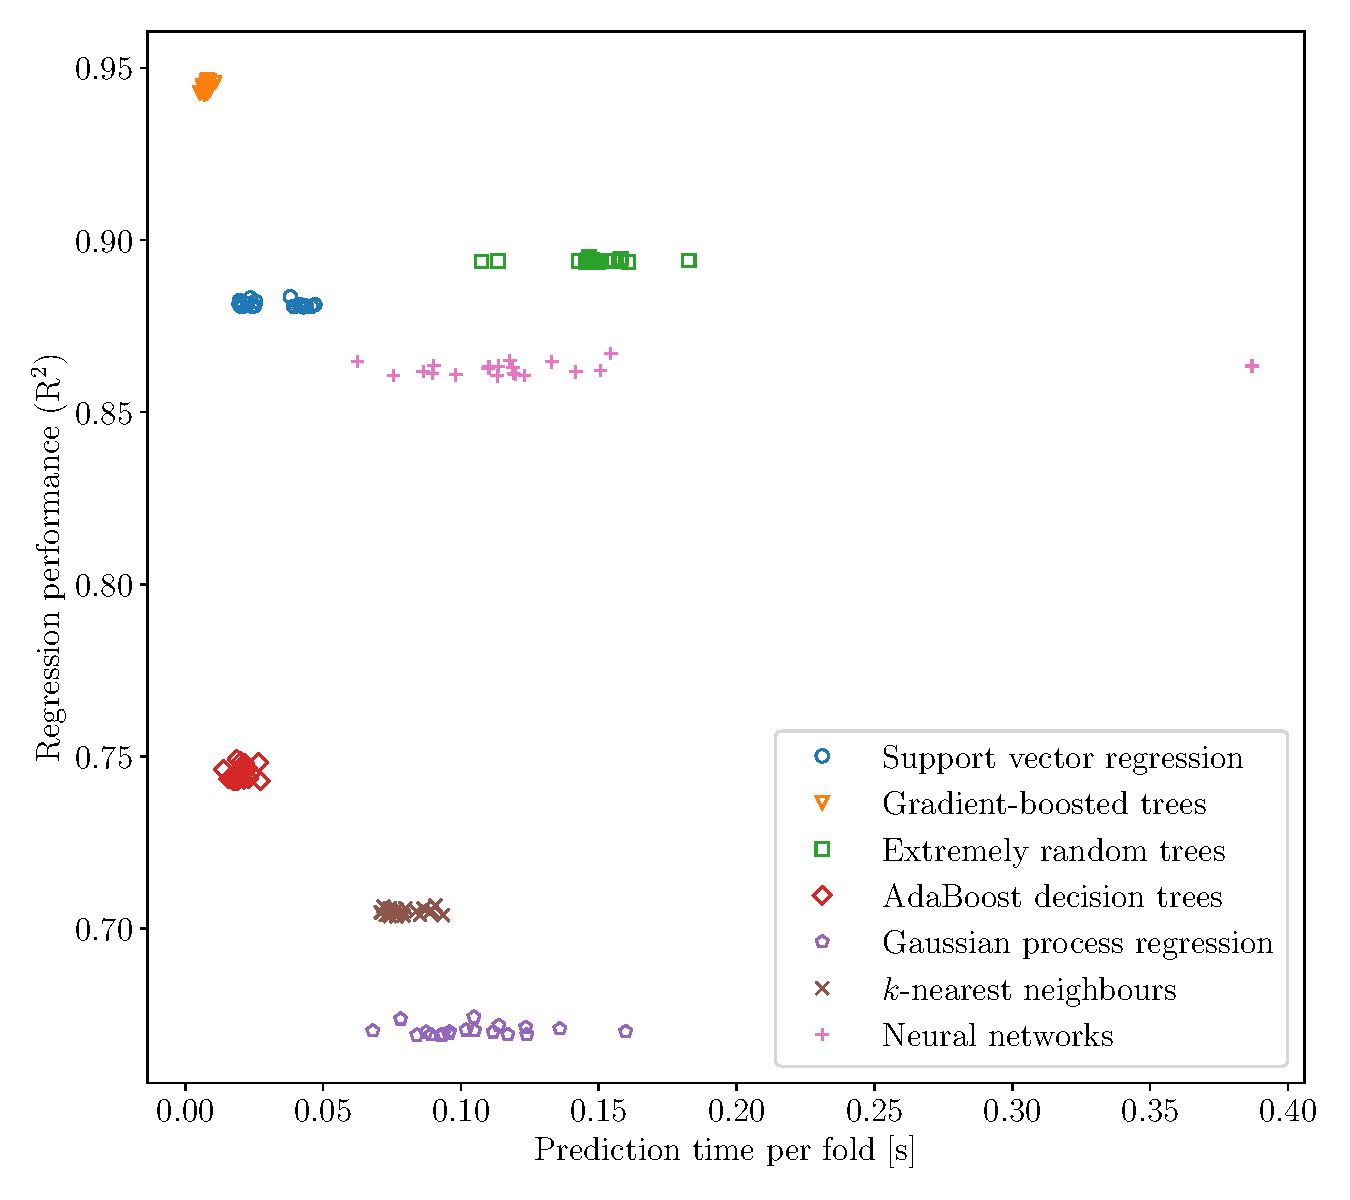
\includegraphics[width=\linewidth]{exp1_time_vs_reg}
		% TODO: only a placeholder, regenerate when data becomes available
		\caption{Experiment 1 (single slice)}
	\end{subfigure}\hfill%
	\begin{subfigure}[b]{0.5\textwidth}
		\centering
		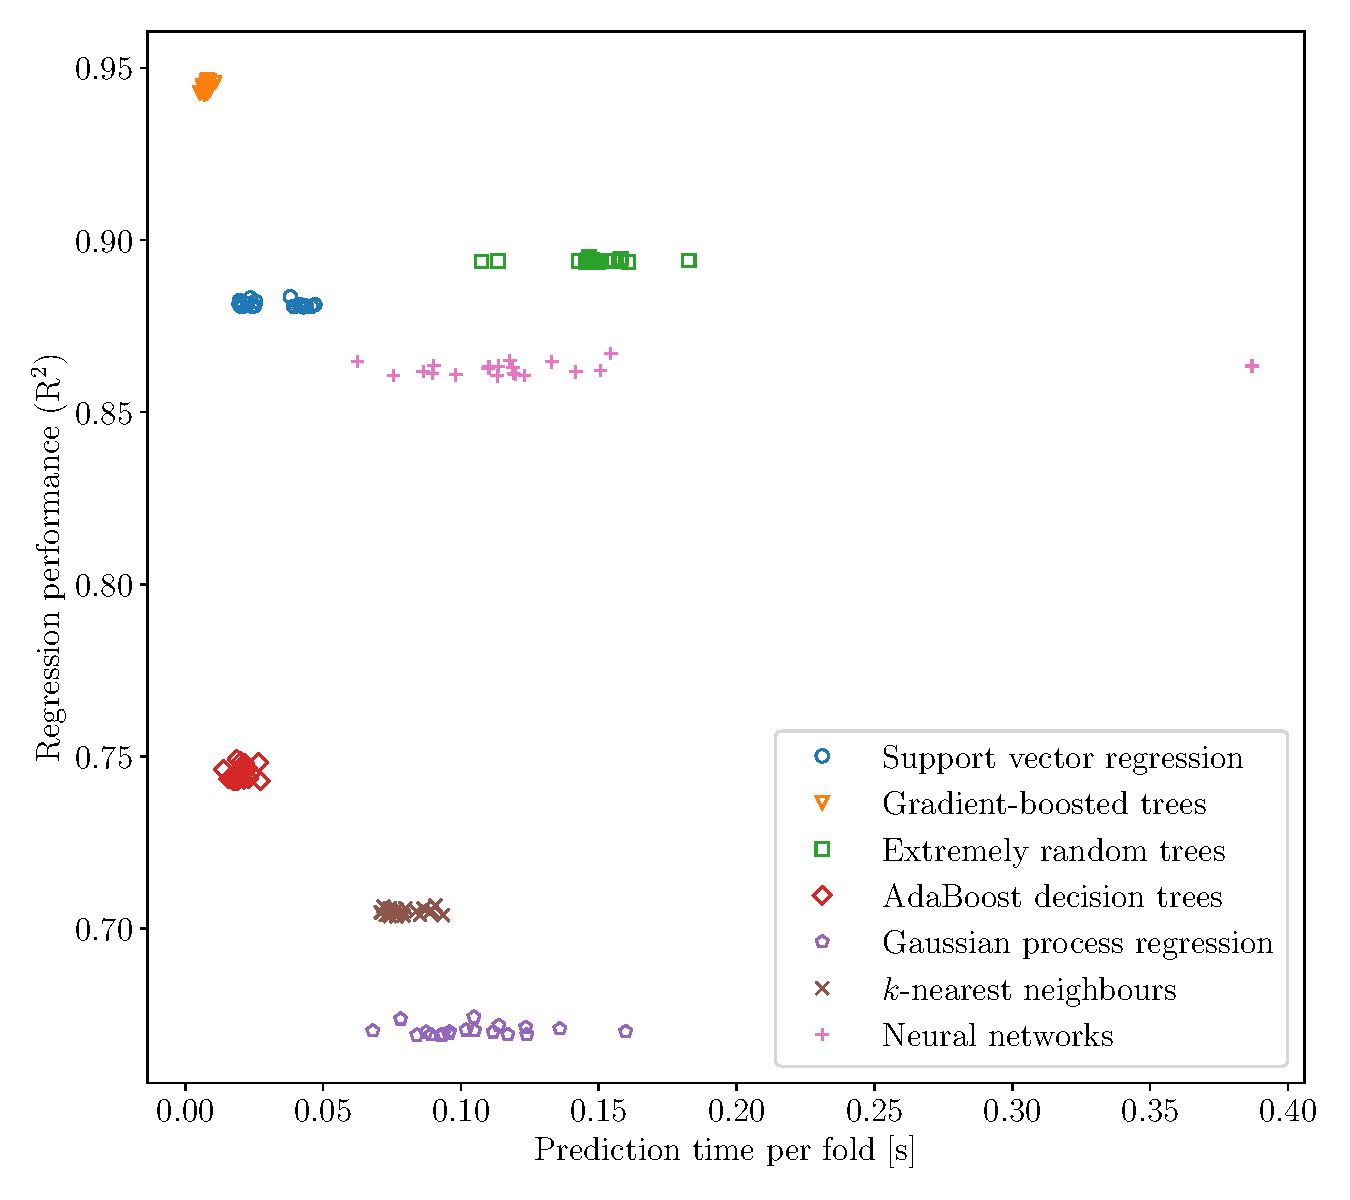
\includegraphics[width=\linewidth]{exp1_time_vs_reg}
		% TODO: only a placeholder, regenerate when data becomes available
		\caption{Experiment 2 (full dataset)}
	\end{subfigure}
	\caption{Regression performance (as $R^2$) plotted against mean
	prediction time for the best $N$~models of each surrogate class.} % TODO. fill N
	\label{fig:time-vs-reg}
\end{figure}


\subsubsection{Scaling Benchmark}

In the next experiment we examine surrogate scaling properties correlating
metrics of interest with progressively increasing training set size. The results
shown in~\cref{fig:scaling} seem to suggest that in terms of regression performance,
methods based on decision trees and neural networks offer the best accuracy on
larger sets overall. This is a curious extension of previous findings, where
gradient boosted trees were observed to significantly dominate over the rest of
the examined methods. With increasing training set size, their relative advantage is
clearly gradually diminished.

\begin{figure}[h]
	\centering
	\begin{subfigure}[b]{0.333\textwidth}
		\centering
		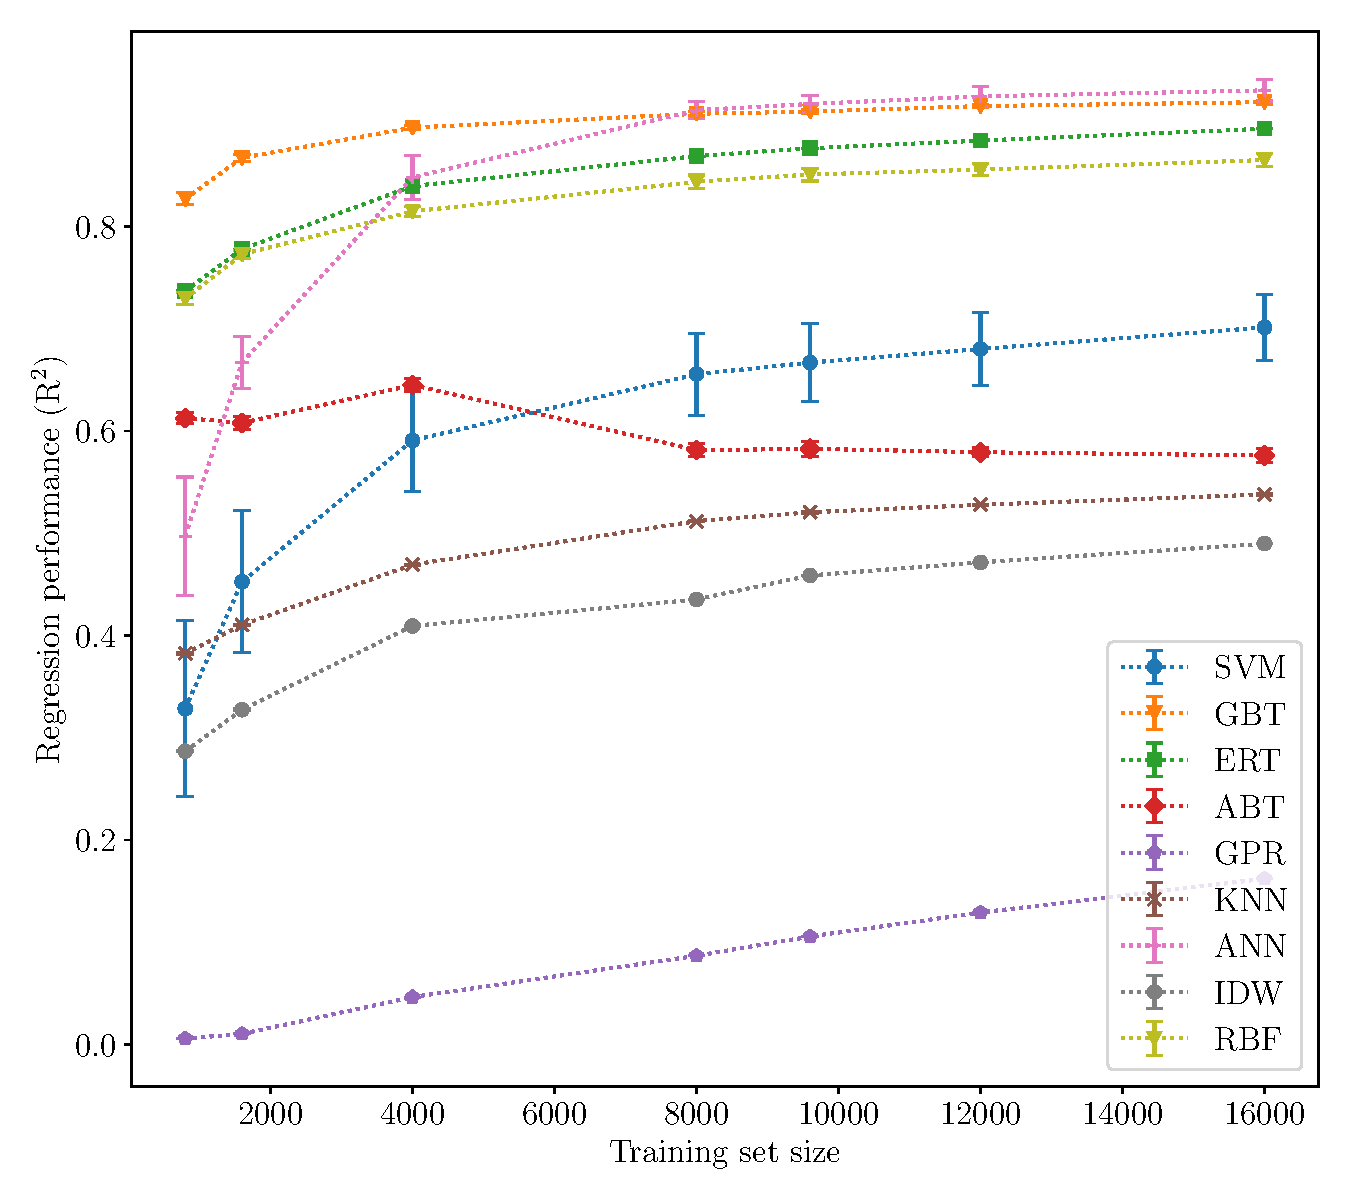
\includegraphics[width=\linewidth]{scaling_metric_r2}
		% TODO: only a placeholder, regenerate when data becomes available
		\caption{Regression performance (as $R^2$)}
	\end{subfigure}\hfill%
	\begin{subfigure}[b]{0.333\textwidth}
		\centering
		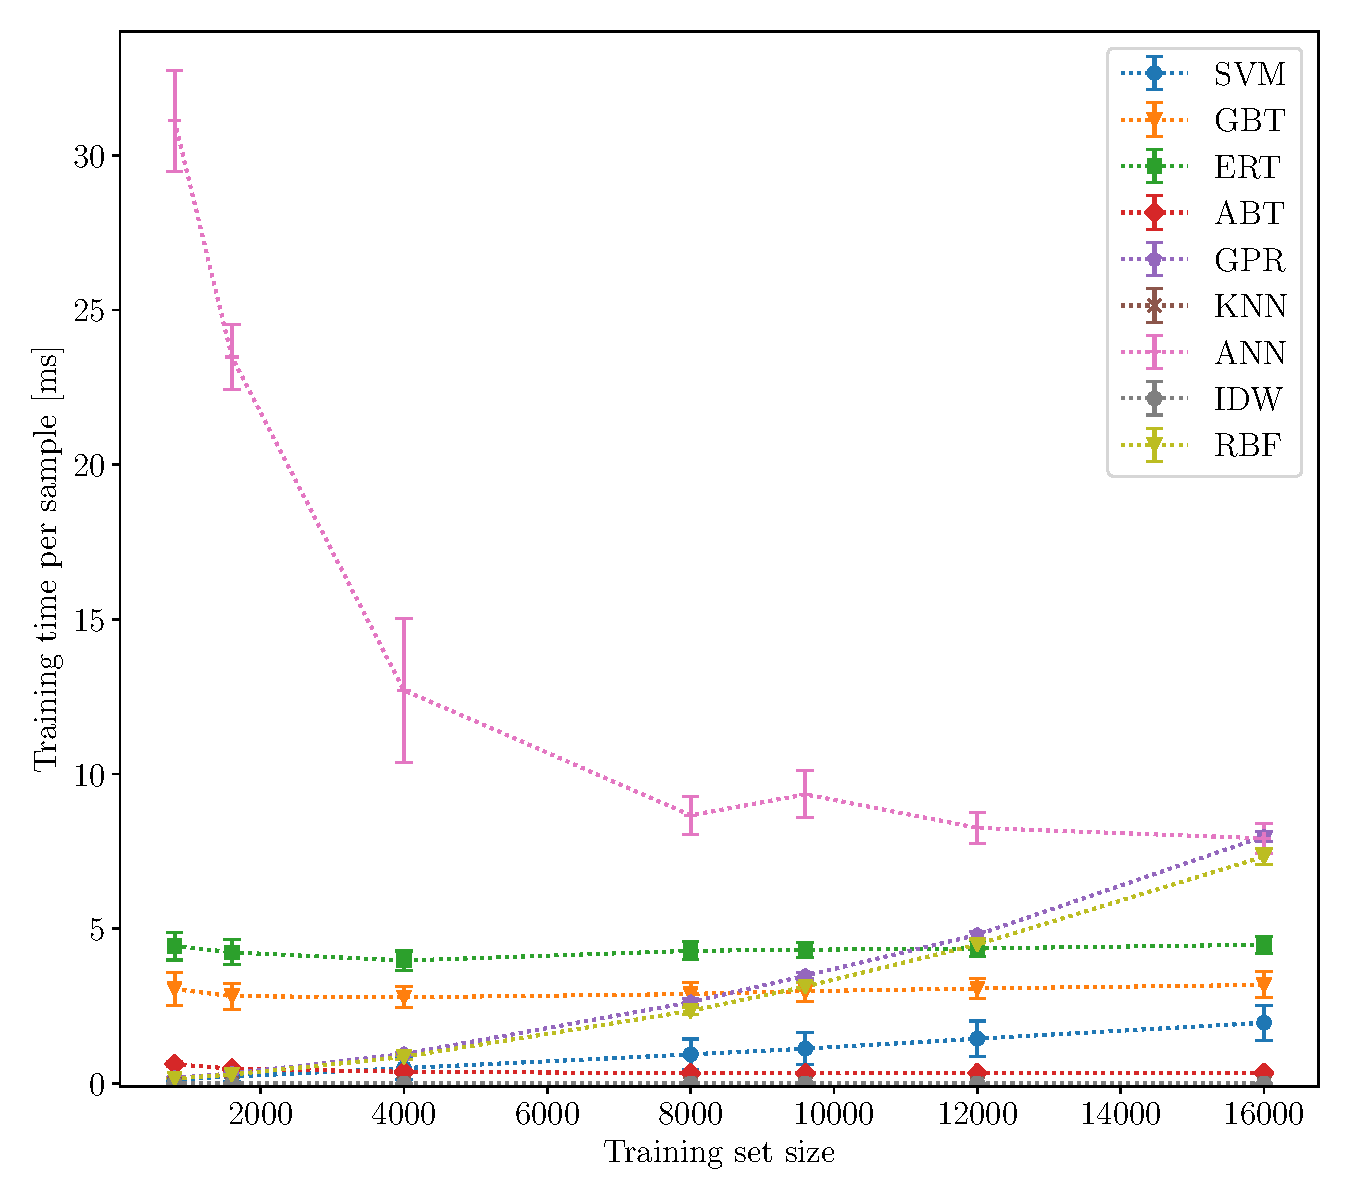
\includegraphics[width=\linewidth]{scaling_time_train}
		% TODO: only a placeholder, regenerate when data becomes available
		\caption{Mean training time}
	\end{subfigure}\hfill%
	\begin{subfigure}[b]{0.333\textwidth}
		\centering
		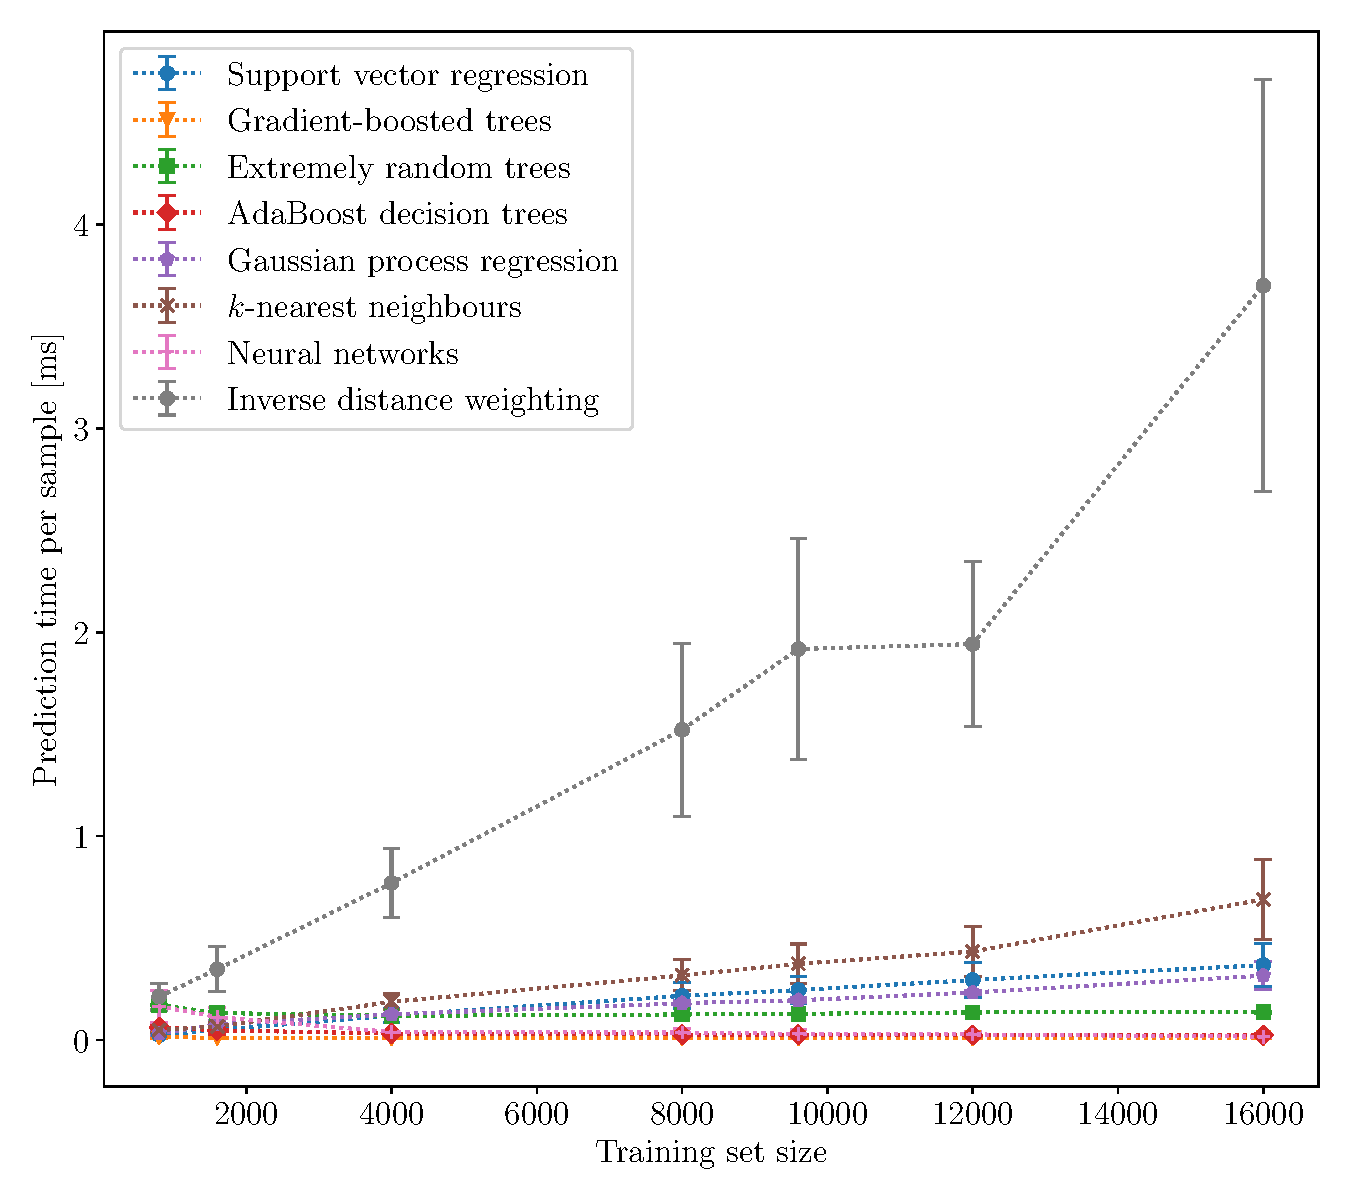
\includegraphics[width=\linewidth]{scaling_time_pred}
		% TODO: only a placeholder, regenerate when data becomes available
		\caption{Mean prediction time}
	\end{subfigure}
	\caption{Various metrics collected during experiment 3 (scaling
	benchmark) displayed as a function of training set size.}
	\label{fig:scaling}
\end{figure}

According to our experiment, the lowest mean training time is generally achieved
by instance-based learning methods, which seem to offer near-constant scaling
characterists at the expense of significant performance increase later during
prediction. Following that, we observe that the majority of tree-based methods also exhibit
desirable properties. The notable exception here appear to be neural networks,
which are the only model to utilise parallelisation. As such, their constant
synchronisation overhead overall hinders performance on small training sets,
producing misleading results when divided by the number of samples.

In terms of mean prediction time, all tested surrogates except previously mentioned
instance-based learning methods scale exceptionally well. Tree-based generally
models appear to perform the fastest.


\subsubsection{Competitive Surrogate Training}

TODO

\begin{figure}[h]
	\centering
	\begin{subfigure}[b]{0.333\textwidth}
		\centering
		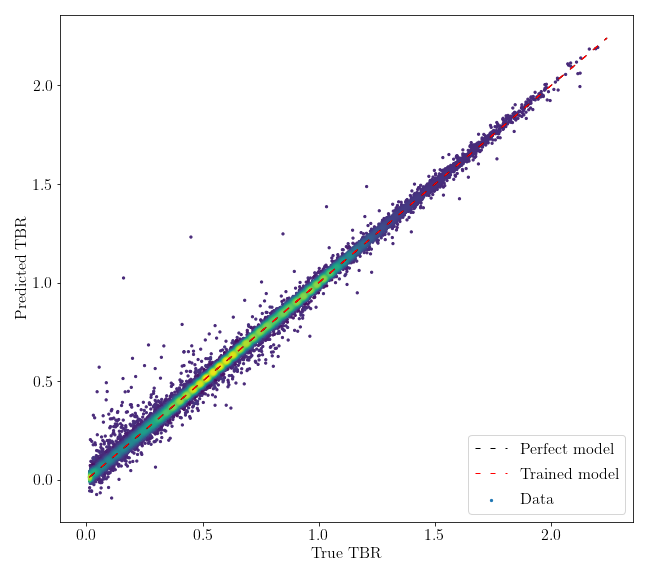
\includegraphics[width=\linewidth]{run1_5ke_1h3f128_4974_performance}
		% TODO: only a placeholder, regenerate when data becomes available
		\caption{Model 1}
	\end{subfigure}\hfill%
	\begin{subfigure}[b]{0.333\textwidth}
		\centering
		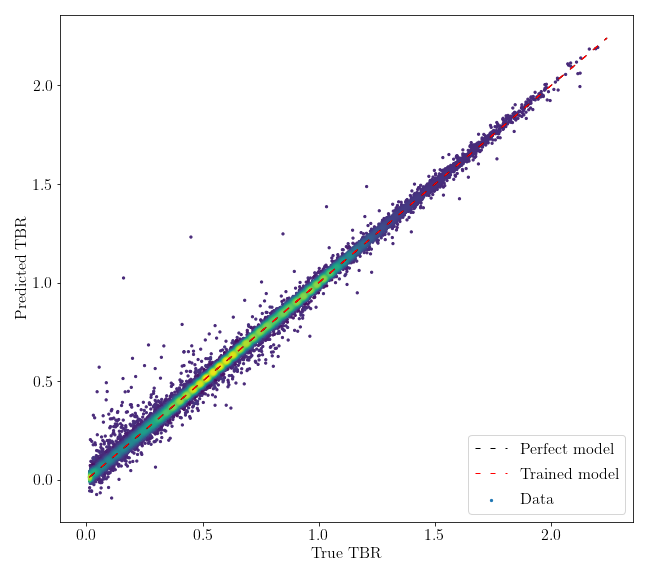
\includegraphics[width=\linewidth]{run1_5ke_1h3f128_4974_performance}
		% TODO: only a placeholder, regenerate when data becomes available
		\caption{Model 2}
	\end{subfigure}\hfill%
	\begin{subfigure}[b]{0.333\textwidth}
		\centering
		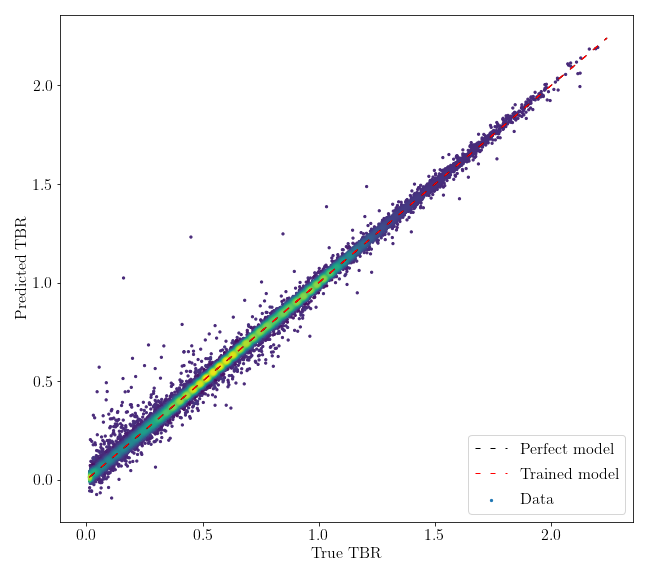
\includegraphics[width=\linewidth]{run1_5ke_1h3f128_4974_performance}
		% TODO: only a placeholder, regenerate when data becomes available
		\caption{Model 3}
	\end{subfigure}

	\vspace{0.75ex}

	\begin{subfigure}[b]{0.333\textwidth}
		\centering
		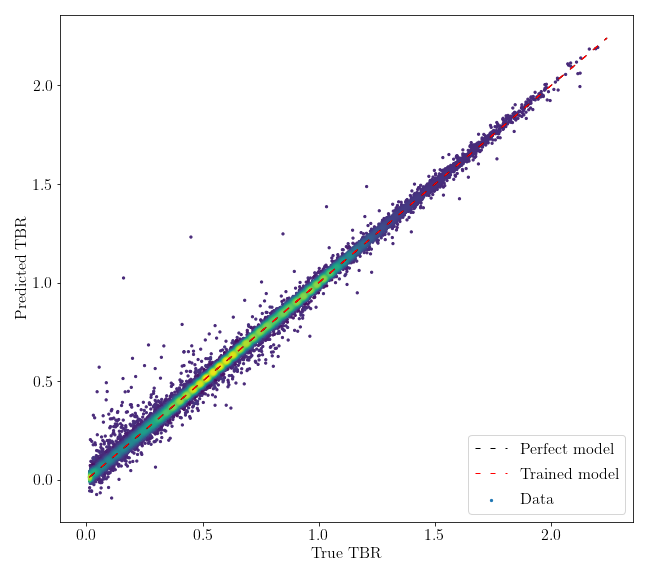
\includegraphics[width=\linewidth]{run1_5ke_1h3f128_4974_performance}
		% TODO: only a placeholder, regenerate when data becomes available
		\caption{Model 1}
	\end{subfigure}\hfill%
	\begin{subfigure}[b]{0.333\textwidth}
		\centering
		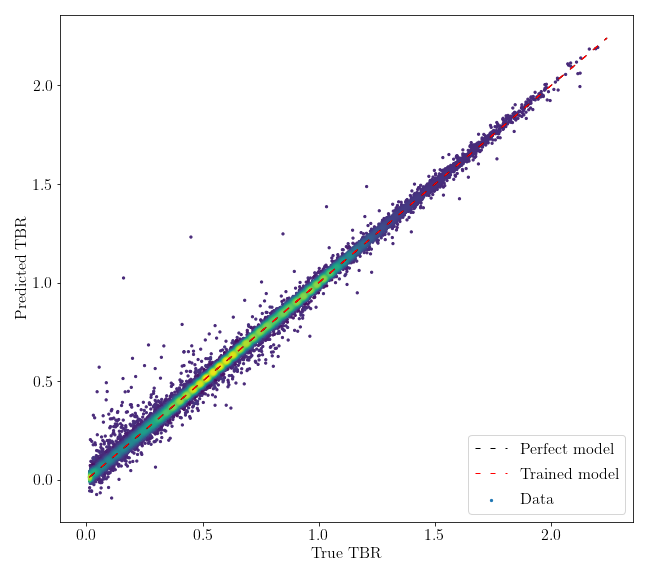
\includegraphics[width=\linewidth]{run1_5ke_1h3f128_4974_performance}
		% TODO: only a placeholder, regenerate when data becomes available
		\caption{Model 2}
	\end{subfigure}\hfill%
	\begin{subfigure}[b]{0.333\textwidth}
		\centering
		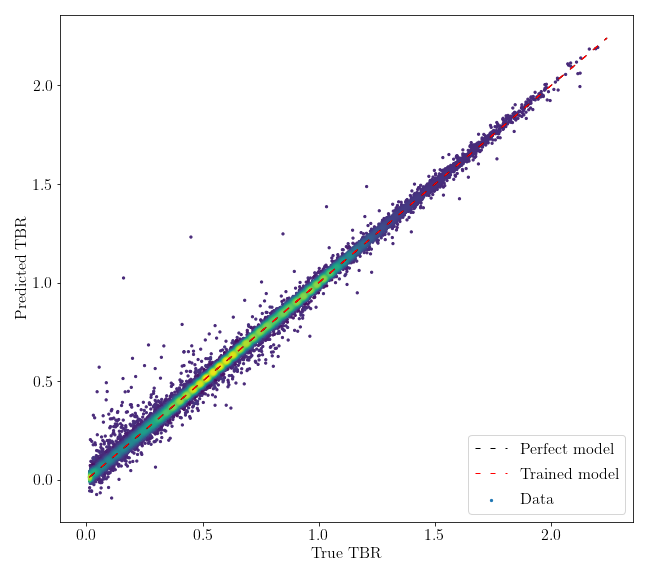
\includegraphics[width=\linewidth]{run1_5ke_1h3f128_4974_performance}
		% TODO: only a placeholder, regenerate when data becomes available
		\caption{Model 3}
	\end{subfigure}
	\caption{Regression performance of the best models trained in experiment~4.}
	\label{fig:reg-performance}
\end{figure}

\subsection{Results of Adaptive Sampling}
\label{sec:adaptiveres}

Define sinusoidal toy model and justify

Explain hyperparameter tests: initsamples, stepsamples, MCMC length

\begin{figure}[h]
    \centering
    \begin{subfigure}[t]{0.5\textwidth}
        \centering
        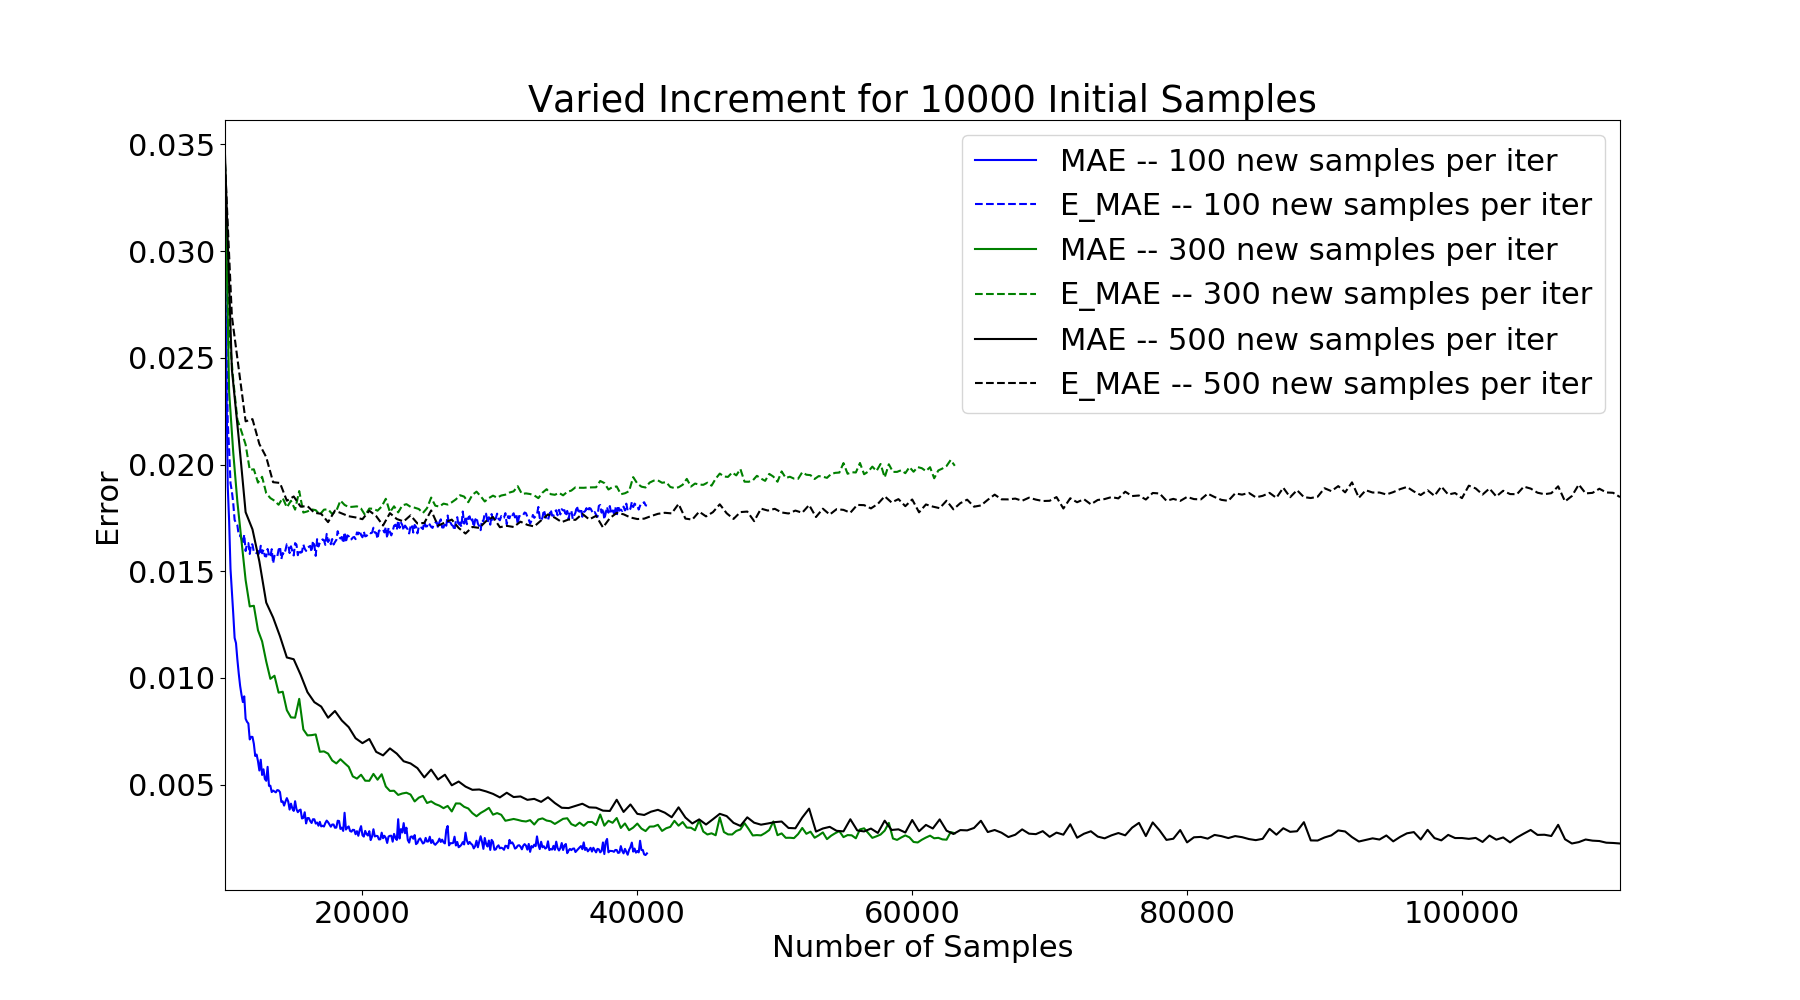
\includegraphics[width=1.1\linewidth]{fig5_qassincrsamp.png}
        \caption{QASS absolute training error over total sample quantity}
    \end{subfigure}%
    ~ 
    \begin{subfigure}[t]{0.5\textwidth}
        \centering
        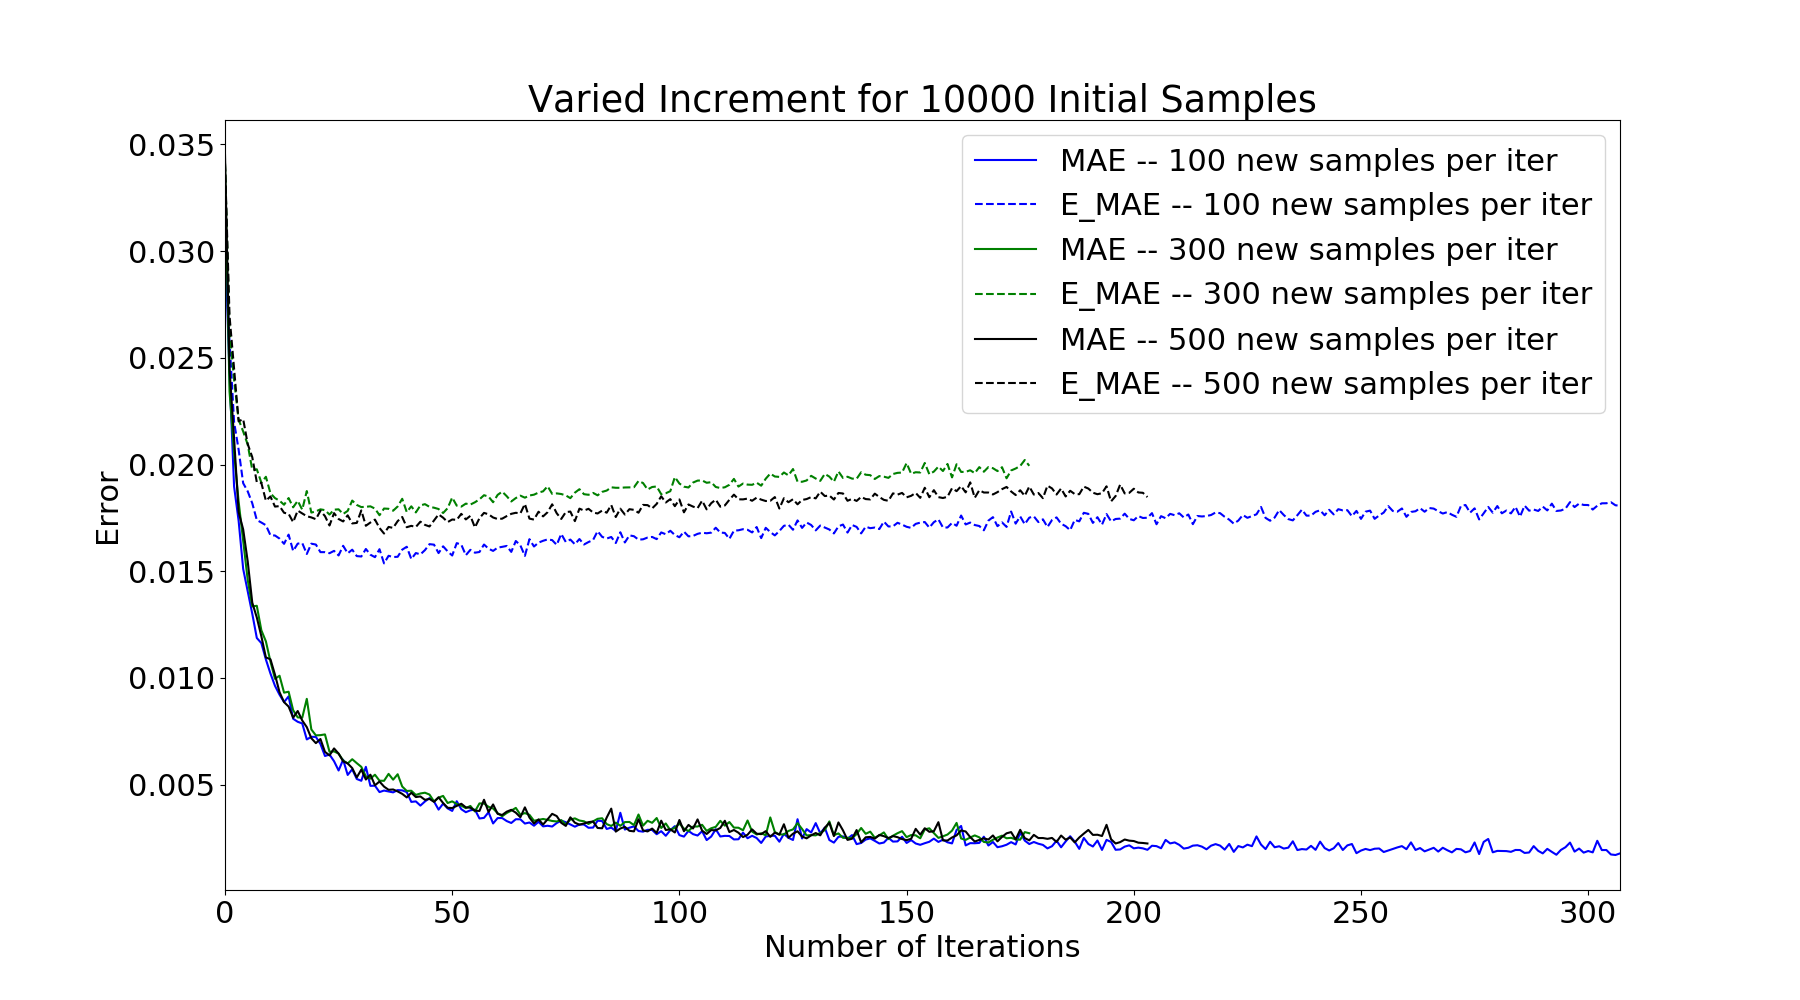
\includegraphics[width=1.1\linewidth]{fig6_qassincrtime.png}
        \caption{QASS absolute training error over number of iterations}
    \end{subfigure}
    \caption{Caption place holder}
\end{figure}

\begin{figure}[h]
  \centering
    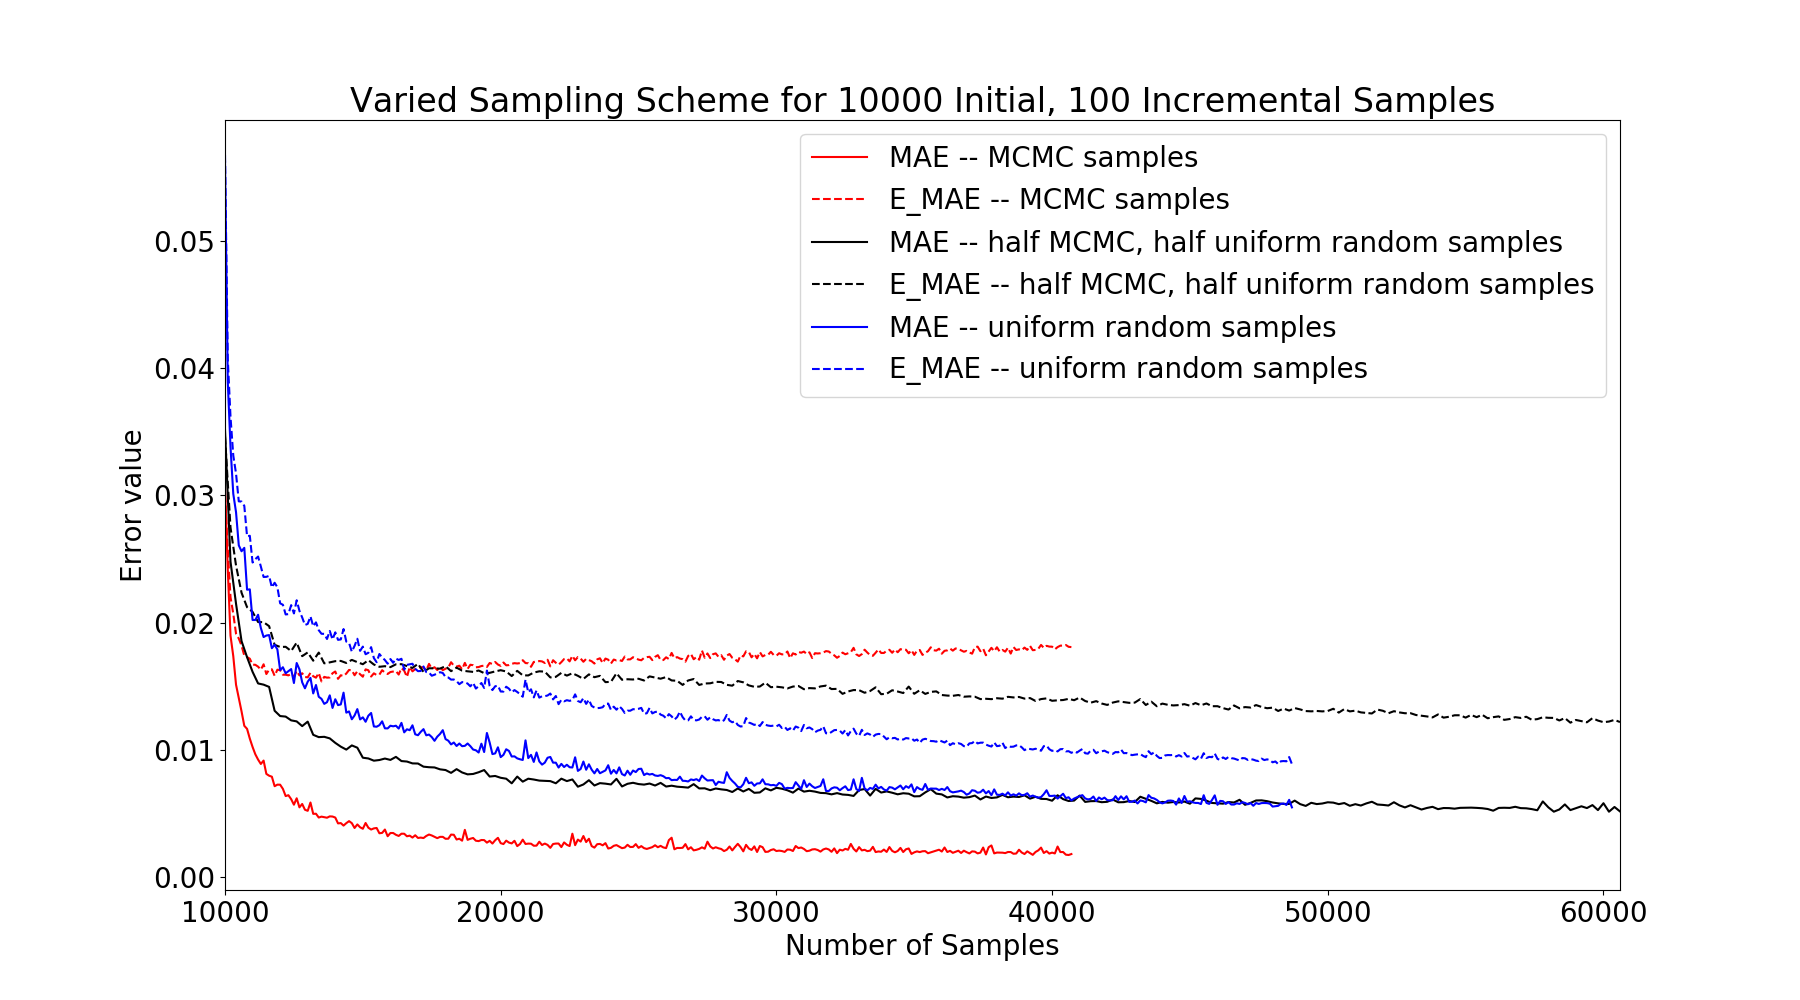
\includegraphics[width=0.8\linewidth]{fig7_qasssampling.png}
    \caption{Absolute training error for QASS, uniform random scheme, and mixed scheme}
  \label{fig:pca}
\end{figure}
